\documentclass{article}
\usepackage{malmacros}
\begin{document}

\section{Regulizers}
This section will explore the power of regulizers. This is used to avoid over-fitting of models. It will constrain (regularize) the model with use of terms such as a \textit{penalty factor}. Furthermore, models such as \textit{ridge} and \textit{lasso} will be discussed that all use this penalty factor.

\subsection{Qa The Penalty Factor}
The penalty factor is used to penalize the flexibility of a model. This is used to reduce over-fitting of a model. 
\\ \\
The penalty part of the penalty factor is calculated in this section. The function \textit{Omega()} will take a weight  vector, which will resemble a polynomial of the form $w_0$ $w_1$ $w_2$ .. $w_d$. The first term $w_0$ should be removed. $w_0$ is the bias - a polynomial consists of a constant factor and values that describe the shape and slope of the curve. The bias $w_0$ is removed, since  only the calculation of the penalty factor of itself is wanted. The bias is the outlier that describes the intersection with the vertical axis. If this point is not removed the data set will be biased towards this point.
\\
The factor is simply calculated as the dot product of the weights and the weights transposed. Which leads to the calculation of the L2 norm.

\begin{pyminted}
def Omega(w):
    # Remove bias of w0
    new_w = np.delete(w, 0)
    return np.dot(new_w.T, new_w)
\end{pyminted}

\noindent
The output after calculating the penalty on the following vectors is shown in the output.

\begin{pyminted}
w_a = np.array([1, 2, -3])
w_b = np.array([1E10, -3E10])
w_c = np.array([0.1, 0.2, -0.3, 0])
\end{pyminted}

\begin{pyconsole}
P(w0)=13
P(w1)=9e+20
P(w2)=0.13
\end{pyconsole}

The penalty is calculated as 13, 9e+20 (a very high number ..) and  0.13 for the three arrays. It can be seen that the vector $w_a$ has a penalty of 13. It is calculated based on the polynomial function of the weights. It shows that the penalty is not too high for this one. Obviously, the third array will be 1/10 of this, since it is simply the same values as the first, just 1/10th of these. The second vector, however, has a very high penalty, since it is a linear line with a very high negative slope. The other two are inverse parabolic functions.

\subsection{Qb Explain the Ridge Plot}
This section will explain the Ridge Plot, and briefly explain the code (will not be inserted here, just explained). the code in this section will take in a model class and 3 different alpha-value (0, $10^{-5}$ and 1). The code iterates through the 3 alpha values and generates a new model (Ridge, Lasso, Elasticnet) and plots these in a figure. This section will only talk about the Ridge model. The ridge model is shown in figure \ref{fig:reg_a}.

\begin{figure}[H]
  \centering
    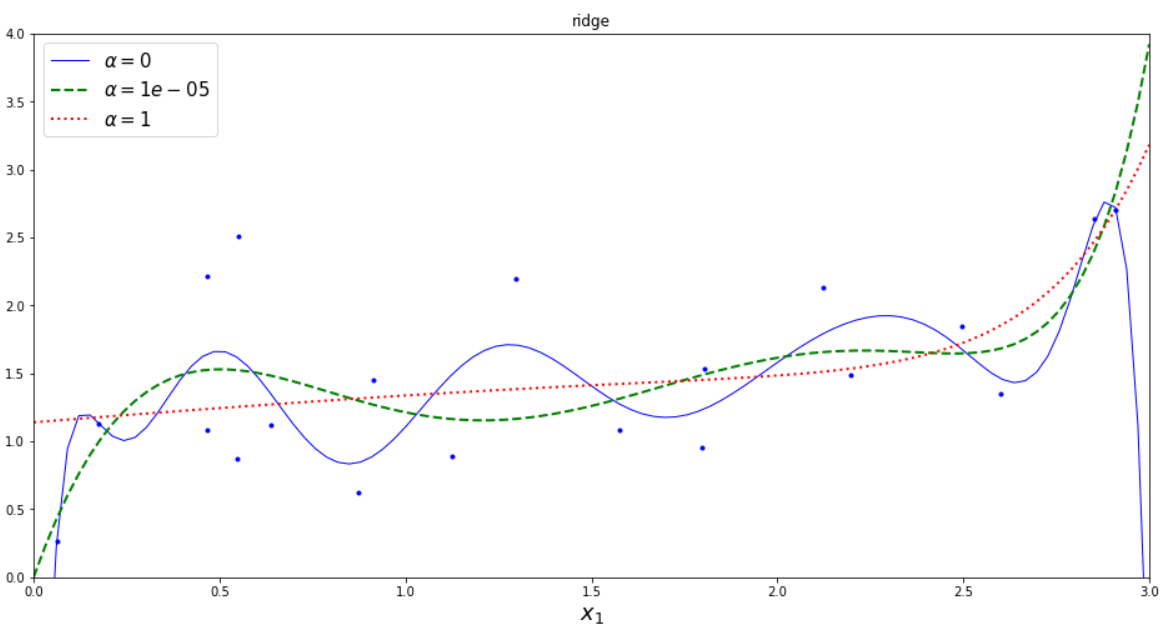
\includegraphics[width=1\textwidth]{les6-reg-b}
    \caption{Ridge model with a = 0, a = 1e - 05, a = 1}
    \label{fig:les6-reg-b}
\end{figure}

The hyperparameter \textit{alpha} (hereafter just written as\textit{a} for simplicity) will control how much the model is regularized. If a = 0, it will just be seen as a Linear Regression. If it is large, then it will  become a line going through the mean. Ridge uses L2 as the norm of the weight vector. 
\\
So when a = 0, it is simply the line itself with no penalty. With a = 1e - 05, some penalty has been added to smoothen out the  curve a bit. Though with a = 1, the curve is much more exponential looking and smoother, but obviously does not follow the points as much as the previous two models does. It will go through the points, closer to the mean of the values.

\subsection{Qc Explain the Ridge, Lasso and ElasticNet Regulized Methods}
% Asbjørn

\paragraph{Ridge regression} is a regularized version of linear regression, where a \textbf{regularization term} is added to the cost function. This regularization term constrains the learning algorithm, as to better fit the data as well as keeping the models weight as small as possible. This is adjusted by changing the chosen \textbf{alpha} values. Keeping \textbf{alpha} = 0 just leaves us with plain old Linear Regression.
But setting \textbf{alpha} to high value will force it towards flat lining through the data. By increasing the the \textbf{alpha} value the models susceptibility to variance is decreased by as always this comes with the trade-off of the added bias.

\paragraph{Lasso Regression} which is short for the long name: Least Absolute Shrinkage and Selection Operator Regression. Is also a regularized version of Linear regression. And it also comes with an added \textbf{regularization term}, but it uses the L1 norm to constrain the model weights, which is opposite to the Ridge regression that uses the L2 norm. Because of this it tends to zero out weights of least importance, which means weights that are close to zero. This gives Lasso regression the trait of automatically performing \textit{feature selection} and creating a more \textit{sparse model} with few non-zero feature weights.

\paragraph{Elastic Net} is a middle ground of both \textbf{Lasso regression} and \textbf{Ridge regression}. It also comes with a \textit{Regularization Term}, which is a mix-in of the two previous models. The mix is controlled by a ratio \textbf{r}, which decides how the regularization should be decided. When \textbf{r} = 0, \textbf{Elastic Net} is equivalent to Ridge regression, using the L2 norm. And when \textbf{r} = 1 its equivalent to Lasso regression.
 
\subsection{Qd Regularization and Overfitting}
% Skal muligvis rettes / kortes lidt ned.
The tug of war between the weighted values defined by the penalty factor and the positioning of the values,
is best explained by first looking at the circles above from a different angle. When we talk about Gradient descent we usually look at bowl. And looking at the circles we simply look at the bowl from above.
Now what the elongated circles represent is where the weighted values after each epoch is placed. 
The inner most circle being the area neares to the global minium.
\\\\
The other circle is the derivative of the weighted values, and are defined by the penaltyfactor which is added to the values.The issue is that depending on the weights and how big the steps are each epoch, the values might jump more, and possibly displace the output values slightly, so that the outcome is slightly skewed. The penalty factor, is added to correct the outcome, and keep them within the right factor, and near the true outcome.
\\ \\
A way to look at it could be if one of the values in the output represented by a X,Y coordinate value,
they could perhabs both be positive values. But the real values or the "true" outcome could be different.
Perhabs lower on the y-axis, maybe even in the negatives, so that the real placement is below the x-axis.
The tug of war between the MSE weighted cost function and the regulization penalty factor,
helps prevent the data from becomming skewed. Unless the regulizer term is too small then the data could pull to far from origin.

\end{document}